\chapter{Numerische Lösungsmethoden}
Nichtlineare Differentialgleichungen sind im Allgemeinen nicht analytisch
lösbar. D.h.\ es ist nicht möglich eine geschlossene Lösung anzugeben. Daher
ist es sinnvoll, sich mit numerischen Lösungsmethoden zu beschäftigen.  Wir
wollen hier nur eine begrenzte auswahl ansprechen. Für ingneieurstechnische
Anwendungen steht ganz klar das Verhältnis zwischen Aufwand für deren
Erarbeitung und Genauigkeit der Ergebnisse im Vordergrund. Deshalb gibt es
keine absolute Aussage, welche Methode die beste ist.

Wir gehen von einem Anfangswertproblem einer Differentialgleichung 1. Ordnung
und 1. Grades aus, wobei hierin auch System erster Ordnung eingeschlossen
seien. Wir schreiben das Anfangswertproblem eines Systems, wie es in
(\ref{eq:NLDGLSystem}) dargestellt ist als
\begin{align}
  \dot{\mathbf{y}}(t) =& \mathbf{f}(\mathbf{y}(t),t) \label{eq:yNLSystem}\\
  \mathbf{y}(0)       =& \mathbf{y}_{0}\nonumber
\end{align}
\section{Die Eulersche Methode}
Wir nehmen an $y(t)$ sei gekannt, dann können wir $y(t+\Delta t)$ in eine
Potenzreihe entwickeln und erhalten bei Vernachlässigung aller Terme 2. und
höherer Potenzen in $\Delta t$ 
\begin{equation}
  y(t+\Delta t) = y(t)+\Delta t f(y(t),t)+O(\Delta t^2),
  \label{eq:Euler}
\end{equation}
wobei $O(\Delta t^2)$ für quadratische und höhere Terme steht.

\begin{note}{Fehler}
  Keine Angabe eines Algorithmus zur Lösung einer DGL ist sinnvoll, wenn nicht
  gleichzeitig auch zumindest die Fehlerordnung, wenn nicht gar der lokale
  Dikretisisierungsfehler angegeben ist.
\end{note}
Wie groß ist der Fehler, den wir bei der Lösung machen, wenn wir
(\ref{eq:Euler}) für gleiche Zeitabstände zu diskreten Zeitpunkten
$t_i$ anwenden? Zumindest in einem Zeitschritt gelingt uns sofort eine Aussage.
Angenommen $Y_i$ sei die exakte Lösung der Differentialgleichung zum Zeitpunkt
$t_i$. Dann können wir $Y_{i+1}$ ebenfalls durch eine Taylorreihe darstellen
\begin{equation}
  Y_{i+1}=Y_{i}
  +\underbrace{\Delta t \left(\frac{dY}{dt}\right)_i}_{f(Y_i,t_i)}
  +\underbrace{\frac{\Delta t^2}{2}\left(\frac{d^2Y}{dt^2}\right)_i}_{\dot{f}(Y_i,t_i)}+\dots
  \label{eq:TaylorExact}
\end{equation}
Wobei wir jetzt auf der rechten Seite von (\ref{eq:TaylorExact}) $Y_i$ durch
$y_i$ ersetzen und von (\ref{eq:Euler}) die Potenzreihe (\ref{eq:TaylorExact})
abziehen. Damit erhalten wir für den Fehler
\begin{equation}
  y_{i+1}-Y_{i+1}=E_{i+1}=-\frac{\Delta t^2}{2}\dot{f}(Y_i,t_i)O(\Delta t^3)
  \label{eq:LokalerFehler}
\end{equation}
Dies ist der Fehler pro Zeitschritt, auch lokaler Diskretisierungfehler genannt.
\section{Runge Kutta Methode}
Wir gehen von einer zentralen finiten Differenzenformel aus. Das bedeutet, dass
die finite Differenz die Ableitung zum Zeitpunkt $t_i+\frac{\Delta t}{2}$
nähert. Wir erhalten
\begin{equation}
  \frac{y_{i+1}- y_i}{\Delta}=\dot{y}_{i+1/2}= f(y_{i+1/2},t_{i+1/2})
  \label{eq:Midpoint}
\end{equation}
wobei aber $y_{i+1/2}$ unbekannt ist. Dies beschaffen wir uns durch
Vorwärtsintegration um einen halben Zeitschritt $\frac{\Delta t}{2}$, somit
\begin{align*}
  \hat{y}_{i+1/2}=&y_i+\frac{\Delta t}{2}f(y_{i},t_{i})\\
  t_{i+1/2} =& t_i+\frac{\Delta t}{2}\\
  y_{i+1} =& y_{i}+\Delta t f(\hat{y}_{i+1/2},t_{i+1/2})
\end{align*}
Dies ist das sogenannte Runge-Kutta-Schema 2. Ordnung. Wir sehen, dass wir
hier, im Gegensatz zum Euler-Methode die Funktion $f$ zweimal auswerten müssen.

Ein verbessertes Schema ist die Runge-Kutta-Methode 4. Ordnung. Wie der Name
sagt, müssen wir hier die  Funktion $f$ viermal auswerten. Wir erhalten
\begin{align}\label{eq:RK4order}
  y_{i+1} =& y_{i}+\frac{\Delta t}{6}\left( 
    f(y_i,t_i)+2f(\hat{y}_{i+1/2},t_{i+1/2})+2f(\hat{\hat{y}}_{i+1/2},t_{i+1/2})
  +f(\hat{y}_{i+1},t_{i+1})\right)\\
  \hat{y}_{i+1/2}=&y_i+\frac{\Delta t}{2}f(y_{i},t_{i})\nonumber\\
  \hat{\hat{y}}_{i+1/2}=&y_i+\frac{\Delta t}{2}f(y_{i+1/2},t_{i+1/2})\nonumber\\
  \hat{y}_{i+1}=&y_i+\Delta tf(\hat{\hat{y}}_{i+1/2},t_{i+1/2})\nonumber
\end{align}

\section{Mehrschrittmethoden}
Die Idee hinter den Mehrschrittmethoden ist, (\ref{eq:NLDGLSystem}) zwischen
$t$ und $t+\Delta t$ zu integrieren
\begin{equation*}
y(t_{n+s})=y(t_{n+s-1})+\int\limits_{t_{n+s}}^{t_{n+s-1}}f(y(t'),t')dt'
\end{equation*}
Das Integral gilt es nun zu nähern. Wir haben ja bereits Werte für $y(t_i)$ zu
den Zeitpunkten $t_n$  bis $t_{n+s-1}$ berechnet. Wir nehmen  diese um eine
Interpolationsfunktion aufzustellen, die wir nun in den Grenzen von $t_{n+s-1}$
bis $t_{n+s}$ integrieren können. Wir nähern $f(y(t),t)$ z.B. durch ein
Polynom $p(t)$ der Ordnung $s-1$, das wir dergestalt konstruiert haben, dass es an
den Interpolationspunkten mit $f(y(t),t)$ übereinstimmt

Das Interpolationspolynom ist analytisch integrierbar.  Explizit schreiben wir
das folgendermaßen
\[ p(t)=\sum\limits_{m=0}^{s-1}p_m(t)f(y(t_{n+m},t_{n+m}). \]
Hierbei bezeichne $p_m(t)$ ein Polynom, das zum Zeitpunkt $t_{n+m}$ gleich 1
ist und zu allen anderen Zeitpunkten 0. Damit nutzen wir $s$ vorhergehende
Zeitschritte aus. Daher auch der Name Mehrschrittverfahren und hier im
speziellen beschrieben ist die Methode von Adams.
%\subsection{Predictor-Corrector Methode}
%\subsection{Shooting- und Matrixmethode für Randwertprobleme
\section{Finite Differenzen (FD) Operatoren}
Entwickle die Funktion $f(x)$ um $x$:
\[ f(x+h)=f(x)+\frac{\partial f(x)}{\partial x}h+\frac{1}{2!}\frac{\partial^2
f(x)}{\partial x^2}h^2+\ldots+\frac{1}{(n-1)!}\frac{\partial^{n-1}
f(x)}{\partial x^ {n-1}}h^ {n-1} +O(h^n) \]
oder
\[f(x+h)=f(x)+ f(x)' h+\frac{1}{2!} f(x)'' h^2+\ldots+\frac{1}{(n-1)!} f(x)^{(n-1)} h^ {n-1} +O(h^n)\]
wir bezeichnen die Funktionswerte auf dem Gitter mit 
\[\mathbf{Z}=\left\{ z_k\right\}_{k=-\infty}^{\infty}\]
Dann bekommen wir die folgende Liste von operatoren

\begin{tabular}{ll}
Shiftoperator:&	$(\mathcal{E}\ z)_k=z_{k+1}$\\
Vorwärts Differenzoperator:&	$(\Delta_+\ z)_k=z_{k+1}-z_{k}$\\
Rückwärts Differenzoperator:&	$(\Delta_-\ z)_k=z_{k}-z_{k-1}$\\
Zentraler Differenzoperator:&	$(\Delta_0\ z)_k=z_{k+\frac{1}{2}}-z_{k-\frac{1}{2}}$\\
Mittelwertoperator:&	$(\gamma_0\ z)_k=\frac{1}{2}(z_{k+\frac{1}{2}}+z_{k-\frac{1}{2}})$\\
Differentialoperator:&	$(\mathcal{D}\ z)_k=(z^\prime)_k$
\end{tabular}

Eine schematische Darstellung ist in in Fig.\ \ref{fig:opaction} dargestellt.
\begin{figure}[!ht]
	        \begin{center}
                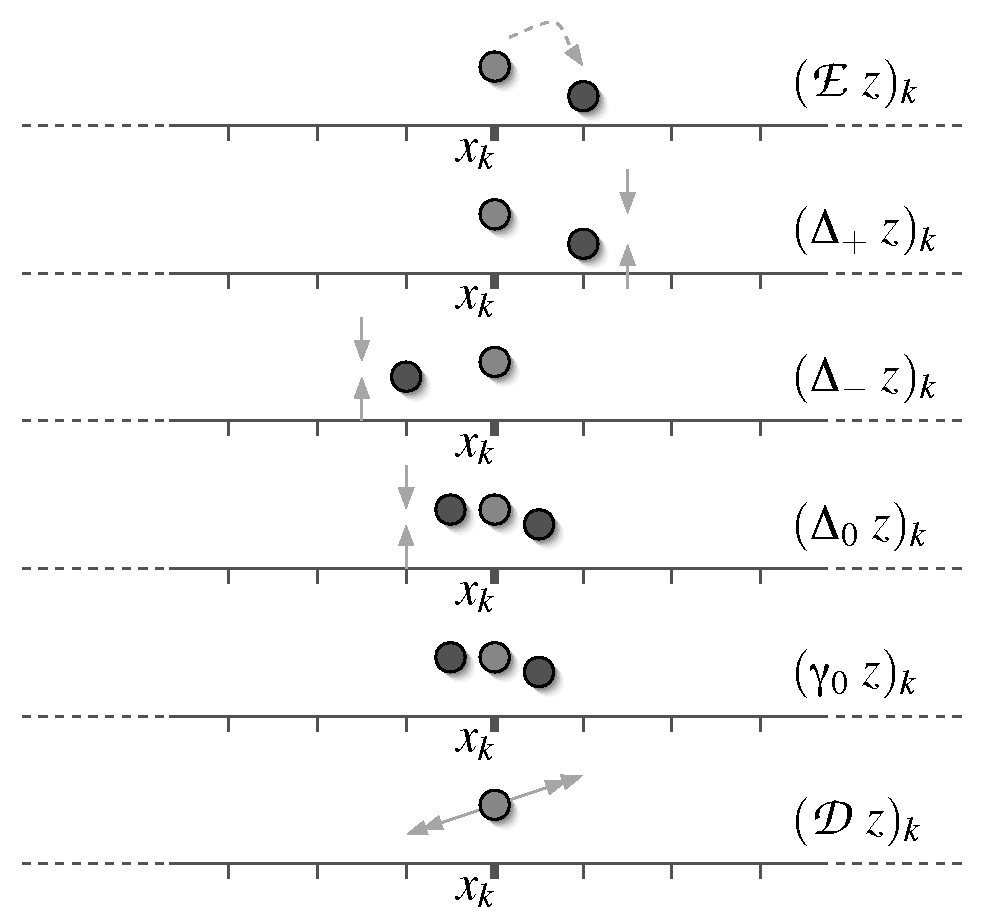
\includegraphics[width=.9\textwidth]{fig/FiniteDifferenceOperators.pdf}
                \caption{Schematic representation of operator actions.\label{fig:opaction}} 
        \end{center}
\end{figure} 

Durch eine Reihenentwicklung des Shiftoperators erhalten wir den Asudruck
für den Differentialoperator
\[
\mathcal{E}z(x)=z(x+h)=\sum_{j=0}^\infty \frac{1}{j!}
\left[{\frac{d^jz(x)}{dx^j}}\right]h^j=
\left[{\sum_{j=0}^\infty}\frac{1}{j!}(hD)^j\right]z(x)=e^{hD}z(x)
\]
womit wir shreiben können
\[ D=\frac{\ln(\mathcal{E})}{h}\]
Beachte, dass Funktionen von Operatoren nur über deren Reihenentwicklung
definiert sind.  Es ist möglich alle Finiten Differenzenopertoren durch den
Shiftoperator auszudrücken:

\begin{tabular}{ll}
	Shiftoperator:&   $(\mathcal{E}\ z)_k=z_{k+1} $\\
	Vorwärts Differenzoperator:&       $(\Delta_+\
	z)_k=z_{k+1}-z_{k}=\left( (\mathcal{E}-\mathcal{I})\ z \right)_k$\\
	Rückwärts Differenzoperator:&     $(\Delta_-\ z)_k=z_{k}-z_{k-1}=
	\left( (\mathcal{I}-\mathcal{E}^{-1})\ z \right)_k$\\
	Zentraler Differenzoperator:&       $(\Delta_0\
	z)_k=z_{k+\frac{1}{2}}-z_{k-\frac{1}{2}}=\left(
	(\mathcal{E}^\frac{1}{2}-\mathcal{E}^{-\frac{1}{2}})z \right)_k$\\
	Mittelwertoperator:&        $(\gamma_0\
	z)_k=\frac{1}{2}(z_{k+\frac{1}{2}}+z_{k-\frac{1}{2}})
	=\frac{1}{2}\left(
	(\mathcal{E}^\frac{1}{2}+\mathcal{E}^{-\frac{1}{2}})z \right)_k$\\
	Differentialoperator:&    $(\mathcal{D}\ z)_k=\frac{1}{h}\left(
	(\ln[\mathcal{E}])z \right)_k$ 
\end{tabular}

Somit erhalten wir für den Differentialoperator

\[
\mathcal{D}=\frac{1}{h}\ln[\mathcal{I}+\Delta_+]=
\frac{1}{h}\left({\Delta_+-\frac{1}{2}\Delta_+^2+
\frac{1}{3}\Delta_+^3 +O\left(\Delta_+^4\right)}\right)
\]
\section{FD für die Lösung von PDEs}
Wir formulieren die FD Form der partiellen Ableitungen auf einem regulären 2D
Gitter, wie z.B. in Fig.\ \ref{fig:gridfd2d} dargestellt.

\begin{figure}[!ht]
        \begin{center}
	        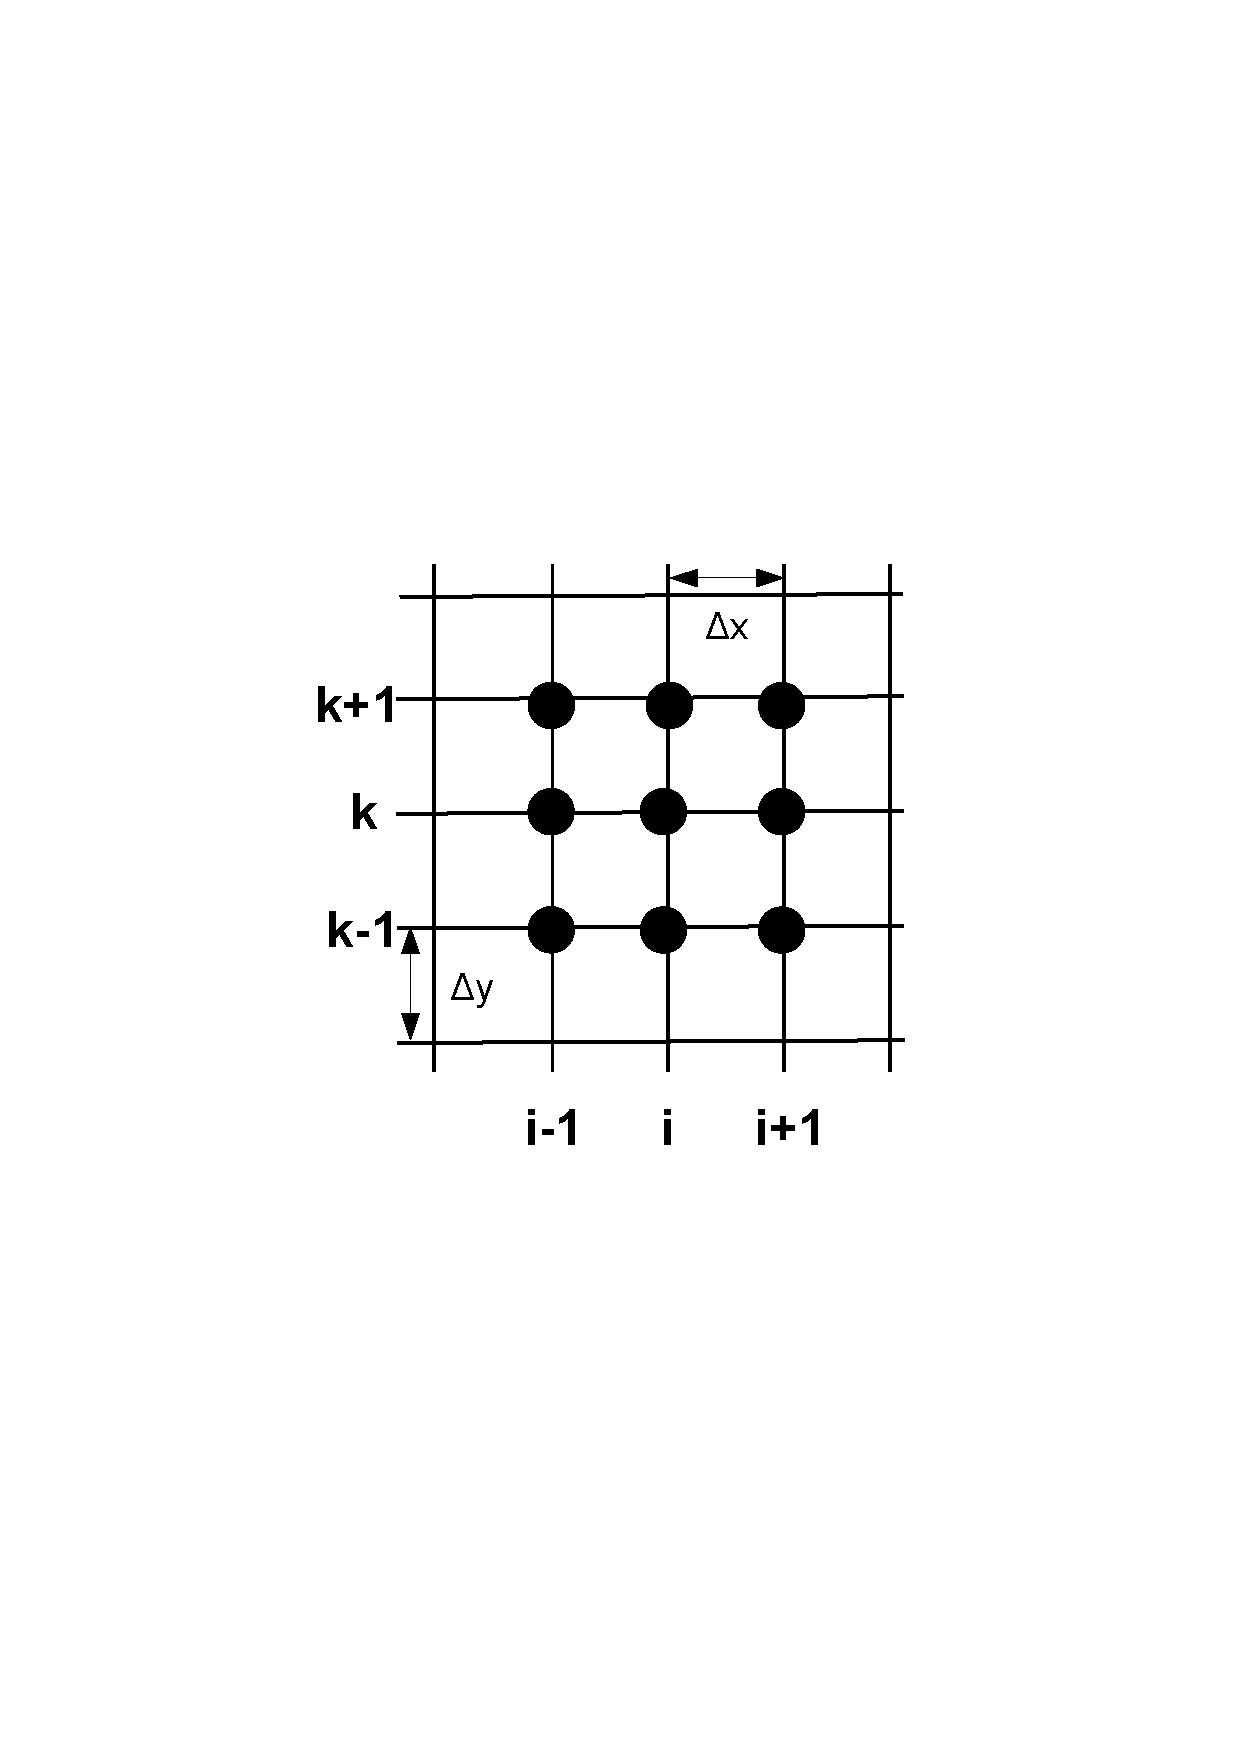
\includegraphics[width=.7\textwidth]{fig/GridFD2D.pdf}
        	\caption{2D FD regular grid.\label{fig:gridfd2d}}
        \end{center}
\end{figure}

Erste und zweite Ableitung auf em Gitter lauten (verify through Taylor expansion!):
\begin{eqnarray*}
	\left(\frac{\partial f}{\partial x}\right)_{i,k}&=&\frac{f_{i+1,k}-f_{i-1,k}}{2\Delta x}\\
	\left(\frac{\partial f}{\partial y}\right)_{i,k}&=&\frac{f_{i,k+1}-f_{i,k-1}}{2\Delta y}\\
	\left(\frac{\partial^2 f}{\partial x^2}\right)_{i,k}&=&\frac{1}{\Delta
	     x^2}(f_{i+1,k}-2f_{i,k}+f_{i-1,k})\\
	\left(\frac{\partial^2 f}{\partial y^2}\right)_{i,k}&=&\frac{1}{\Delta
	     y^2}(f_{i,k+1}-2f_{i,k}+f_{i,k-1})\\
	\left(\frac{\partial^2 f}{\partial x\partial y}\right)_{i,k}&=&\frac{1}{4\Delta x\Delta
	     y}(f_{i+1,k+1}-f_{i+1,k-1}+f_{i-1,k-1}-f_{i-1,k+1})
\end{eqnarray*}
\begin{example}{Laplacegleichung 2D}
Wie lautet die diskrete Form der Laplacegleichung
\[
\left(
\frac{\partial^2}{\partial x^2}+\frac{\partial^2}{\partial x^2}
\right)u(x,y)=0
\]
mittels der Finiten Differenzen Methode?
\end{example}